\documentclass[aps, prc, reprint, amsmath, groupedaddress, nofootinbib]{revtex4-1}
\usepackage[compat=1.1.0]{tikz-feynman}
\usepackage[utf8]{inputenc}
\usepackage{hyperref}
\usepackage{amsmath}
\usepackage{amssymb}
\usepackage{amsfonts}
\usepackage{tabularx}
\usepackage{booktabs}
\usepackage{graphicx}
\usepackage{color}
\usepackage{multirow}
\usepackage{verbatim}
\usepackage[inline]{enumitem}
\graphicspath{{fig/}}
\definecolor{theblue}{RGB}{0,50,230}
\usepackage{appendix}
\hypersetup{
  colorlinks=true,
  linkcolor=theblue,
  citecolor=theblue,
  urlcolor=theblue
} 


\newcommand{\trento}{T\raisebox{-0.5ex}{R}ENTo}
\newcommand{\nch}{N_\text{ch}}
\newcommand{\sqrts}{\sqrt{s_{NN}}}
\newcommand{\T}{\tilde{T}}
\newcommand{\paddedhline}{\noalign{\smallskip}\hline\noalign{\smallskip}}
\newcommand{\dnchdy}{dN_\text{ch}/d\eta}
\newcommand{\dndypP}{dN_\text{pPb}/d\eta}
\newcommand{\dndyPP}{dN_\text{PbPb}/d\eta}
\newcommand{\x}{\mathbf x}
\newcommand{\y}{\mathbf y}
\newcommand{\z}{\mathbf z}
\newcommand{\trans}{^\intercal}

\newcommand{\Raa}{R_{AA}}
\newcommand{\vv}{v_2\{2\}}
\newcommand{\vvv}{v_3\{2\}}
\newcommand{\vnv}{v_n\{2\}}
\newcommand{\ppi}{\frac{\partial}{\partial p_i}}
\newcommand{\ppj}{\frac{\partial}{\partial p_j}}
\newcommand{\ppl}{\frac{\partial}{\partial p_l}}
\newcommand{\Kpara}{\kappa_{\|}}
\newcommand{\Kperp}{\kappa_{\perp}}
\newcommand{\Ppara}{\hat{P}^{\|}}
\newcommand{\Pperp}{\hat{P}^{\perp}}

\begin{abstract}
In relativistic heavy-ion collisions, the heavy flavor production at high transverse momenta are strongly suppressed compared to proton-proton collisions and an unexpected large azimuthal anisotropy was found for charmed meson in non-central collisions. 
Both observations pose challenges to the theoretical understanding of the coupling between heavy quark and the quark-gluon plasma.
The linearized Boltzmann transport and the Langevin equations are two widely used kinetic models for heavy quark in-medium propagation.
In this work, we develop a hybrid transport model that combines the strengths of both: 
heavy quarks scatters with medium partons through perturbative matrix-elements, while between scatterings heavy quarks are evolved with Langevin equations using empirical transport coefficients.
The diffusion constant parametrizes interactions that may be missing in the leading order perturbative scattering picture.
Both elastic and inelastic processes are included in the scattering component.
The Landau-Pomeranchuk-Migdal effect is treated effectively via gluon formation time and detailed balance is imposed for inelastic processes between gluon emission and absorption.
With the hybrid transport model coupled to the state-of-the-art event-by-event bulk evolution generator, we study the heavy flavor azimuthal anisotropy, nuclear modification factor in Pb+Pb collisions at $\sqrt{s} = 5.02$ TeV.
Model parameters are calibrated in a Bayesian approach by systematic comparing to available D-meson and B-meson data at the LHC.
Using the calibrated model, we study the implications on the heavy-flavor transport properties and predict novel observables at the same beam energy.
\end{abstract}


\begin{document}
\title{A hybrid heavy quark transport model in a quark-gluon plasma that couples linear Boltzmann equation and Langevin diffusion dynamics}
\author{Weiyao Ke}
\author{Yingru Xu}
\author{Steffen A.\ Bass}
\affiliation{Department of Physics, Duke University, Durham, NC 27708-0305}
\date{\today}
\maketitle

\section{Introduction}
In recent years, Relativistic Heavy-Ion Collider (RHIC) at Brookhaven National Laboratory and later the Large Hadron Collider (LHC) at CERN discovered a new state of matter, namely the strongly coupled quark-gluon plasma (sQGP), in ultra-relativistic heavy-ion collisions.
Two key signatures in the discoveries of sQGP are the collective flows and the jet quenching.
The collective flows reveal that the bulk medium of sQGP undergoes a strong collective expansion after being produced.
The bulk behavior can be surprisingly explained in great details by models using a relativistic viscous hydrodynamics with the smallest specific viscosity ($\eta/s$) ever discovered in nature.
The jet quenching refers to that the yield of high transverse momentum hadrons in nuclear collisions are strongly suppressed compared to the scaled yield in proton-proton collisions where medium effects are small.
Calculations have shown that this suppression is a consequences of jet losing energy to the hot, dense and color-deconfined medium. 
Open heavy flavors (charm and bottom) as probes of sQGP partly belong to the jet observables but are also special due to their large masses and unique flavors.
Because the temperatures achieved in nowadays experiments are still much smaller than charm and bottom masses, their thermal productions are highly suppressed; 
therefore the dominant production mechanism is the production through hard processes at very early times of the collision.
Also the number of open heavy flavors are roughly conserved during the life time of QGP evolution, because they are dilute probes and seldom annihilate or recombine with their anti-particles.
These two features are particular attractive to theorists as heavy quarks experience the full medium evolution and these flavor-tagged particles are much easier to track in the calculations than the evolution of a full jet.
The mass also sets an additional energy scale to the problem and brings rich physics to the heavy flavor sector.
In the high transverse momentum region, heavy quarks lose energy mainly through radiative process and this merge to the regime of jet energy loss study;
in the low transverse momentum region, mass effect delays its thermalization time \cite{Moore:2004tg}, providing a window to study the equalibration process.
Heavy flavors are therefore ideal and unique probes to study the sQGP properties.

The in-medium propagation of heavy flavors is often studied in a kinetic approach that is linearized with respect to heavy quark distribution function and the medium particle distribution function are assumed to be thermal obtained from hydrodynamic models.
The linearization means any back reactions from heavy quark to the medium are neglected.
Linearized Boltzmann transport equation and Langevin equation are both widely used linearized models but focus on different levels of description of the interaction \cite{Auvinen:2009qm,Cao:2016gvr, Cao:2017hhk, PhysRevD.37.2484, Moore:2004tg}.
The linearized Boltzman transport equation is built on elementary scattering processes that can be directly related to fundamental calculations.
In principal, perturbative Quantum-Chromodynamics (pQCD) can predict the scattering rate of these elementary processes.
However, calculations in the presence of a medium is extremely complicated even at leading order \cite{Arnold:2002zm}.
Also, the pQCD processes are often plagued by soft divergence that need to be regulated by a medium scale proportional to temperature, but with current collision energies the relevant temperature is not high enough that brings large ambiguity to pQCD calculation through the scale dependence of the strong coupling constant $\alpha_s$.
The Langevin equation takes a different perspective. 
It assumes that heavy quark receives frequent but soft momentum kicks from the medium, then a statistical description in terms of ``drag" and ``diffusion" coefficients of the interaction is possible.
These transport coefficients encode the first and second moments of the momentum-exchanging rate but are agnostic to further details of the elementary processes and medium properties.
There are efforts to calculate these transport coefficients in various approaches including lattice QCD evaluations \cite{Moore:2004tg, Gossiaux:2008jv,He:2012df,Riek:2010fk,Ding:2012sp,Banerjee:2011ra}, but for our purposes to understand these properties from experiment data, it is the vast flexibility to parametrize the transport coefficients that the Langevin equation is most useful and we learn these transport coefficients by fitting experiments.
That drawback is vague connection between the fitted phenomenological transport coefficients and a more fundamental understanding of the interaction mechanism.
In this work, we would like to combine the strengths of both approaches
and develop a hybrid heavy quark transport model.
In the hybrid model, the heavy quark scatters off medium particles in a linear Boltzmann equations with pQCD matrix elements (the scattering component), and between scatterings heavy quark is propagated by a Langevin equation (the diffusion component) with empirical transport coefficient mimic the interaction missing from the above scattering picture.
Both elastic and inelastic scatterings are included in the scattering component with soft divergence screened by a Debye mass $m_D$ and Landau-Pomeranchuk-Migdal (LPM) effect taken into account effectively.
The scattering process inside a medium is a multi-scale problem that includes at least a momentum transfer scale $Q$ and a medium scale that is proportional to the temperature $\mu\pi T$.
The QCD strong coupling constant has a scale dependence that we choose to be the maximum of $Q$ and $\mu\pi T$, which means the typical scale of an in-medium process is cut-off by the medium scale.
The details of the running coupling constant we utilized can be found in Appendix \ref{appendix:alphas}.
The medium scale parameter $\mu$ is the only parameter in the scattering component and we assume it encodes the uncertainty in the pQCD matrix-element approach in our models.
The diffusion component have several parameters depending on the way in which transport coefficients are parametrized. 
The idea is to absorb any diffusion-like interaction that is missing from leading order pQCD scatterings into these coefficients.
For example, the diffusion component may include non-perturbative effects.
Also, the effect of small momentum transfer scatterings that may suffer too much from the scale ambiguity is assumed to be compensated by the diffusion component; therefore, the parameters will be correlated with $\mu$ once we tuned the hybrid model to data.
We have noticed that a rigorous separation of matrix-element scattering and diffusion has been proposed for the study of jet energy loss up to next-to-leading order within the context of pQCD \cite{Ghiglieri:2015ala}.
In our study, we don't require the content of the diffusion component to be pQCD in nature.
In fact, we can understand this hybrid approach in the following way, given that a major part of the heavy quark medium interaction is explained by pQCD, what is still needed for the theory to describe the data is parameterized in diffusion component that can be learned from data.

To learn the knowledge in the context of relativistic heavy-ion collisions, we calibrated all model parameters by comparing model to experimental data to see how the system must behave.
The calibration requires evaluating a multi-stage model of the medium plus heavy flavor evolution for arbitrary input parameters in a high dimensional parameter space.
It is almost impossible to tune parameters by hands because of the model complexity and the curse of dimension.
To solve this problem, our field have been developing powerful statistical tools based on Bayesian methodology to conduct systematic model-to-data comparisons \cite{Novak:2013bqa,Bernhard:2015hxa}.
This approach takes experimental uncertainties into account and defines the probability likelihood function of the model parameters given the experimental data.
The Bayesian technique is particularly useful when we are interested in a few or a certain combination of the parameters such as transport coefficients.
It allows marginalization over (to integrate out) other parameters and computes the probability distribution for the parameters of interest. 
The marginalization provides a parameter range that is not only preferred by the experiments, but also already includes uncertainties in the other model parameters.
Therefore the Bayesian technique really tells what can be actually learned from the data, considering both experimental accuracy and model uncertainties.
The Bayesian methodology has been successfully applied to the extraction of initial condition and bulk transport coefficients from soft observables \cite{Novak:2013bqa, Pratt:2015zsa, Bernhard:2015hxa, Bernhard:2016tnd, Auvinen:2017fjw} and to the heavy quark sector extracting heavy quark momentum diffusion parameter $\hat{q}$ using a radiation improved Langevin equation \cite{Xu:2017obm, Cao:2013ita}.
In this work, we provide another extraction of heavy quark transport properties using the hybrid model and also compare with previous works to see how the results dependent on the use of different models.

The paper is organized as follows. 
We describe the hybrid model in detail in section \ref{section:model}. In section \ref{section:test}, the model is tested in a static medium with default parameters. 
We calibrate the model parameters in section \ref{section:calibration} and predict novel observableswith with high likelihood parameter sets in section \ref{section:prediction}. 
Finally, section \ref{section:conclusion} contains summary and discussion of results.

\section{Heavy quark propagation in a hybrid transport model}\label{section:model}
As introduced ioin the prevus section, the hybrid heavy quark transport model consists of a scattering component and a diffusion component.
They are described in details below.
\subsection{Scattering component}
Elementary scatterings of heavy-flavor with medium particles are treated in a linearized Boltzmann equation,
\begin{eqnarray}
  \frac{\partial}{\partial t}f_Q - \frac{\vec{p}}{E}\cdot\nabla f_Q  = 
\mathcal{C}[f_Q]
%C_i^{2\rightleftharpoons 2}[f_Q] + C_i^{2\rightleftharpoons 3}[f_Q]
\end{eqnarray}
The left hand side represents free transport of the heavy quark distribution function. 
Scatterings with medium partons change the distribution via the collision integral on the right.
The medium partons are assumed to obey classical statistics for simplicity, whose thermal occupancy number follows the Maxwell--J\"uttner distribution, 
\begin{eqnarray}
f_{q,\bar{q}, g}(t,x,p) = \exp\left(-\frac{p \cdot u(t,x)}{T(t,x)}\right),
\end{eqnarray}
and any off-equilibrium corrections are neglected.
The space-time evolution of the temperature field $T$ and velocity field $u^\mu$ are obtained in an event-by-event 2+1D viscous relativistic hydrodynamic calculation \cite{Heinz:2005bw,Song:2007ux,Shen:2014vra}.
We solve $f_Q(t,x,p)$ in a Monte Carlo way by representing the distribution function with an ensemble of heavy quarks.
Within a given time step $dt$, each heavy quark undergoes scatterings according to its reaction probability $P$.
We always calculate $P$ in the center-of-mass (CoM) frame of local fluid cell defined with temperature $T$ and velocity $u^\mu$.
In this reference frame, the heavy quark with energy $E_1$ can collide with a few medium particles that together forms an $n$-body initial state denoted as $\{\textrm{in}\}$, and the outgoing particles after the collision forms the $m$-body final state $\{\textrm{out}\}$.
The probability for heavy quark undergoes reaction of a certain channel inside the fluid cell per unit time is the so called scattering rate $\Gamma$,
\begin{eqnarray}\label{eq:rate}
    \frac{dP}{dt} &=& \Gamma(E_1, T, t) \nonumber \\
    &=& \frac{d}{\nu} \frac{\delta}{\delta f_Q(p_1)}\int d\Phi(n,m) \prod_{\textrm{\{in\}}} f_i(p_i) 
\overline{|M|^2},
\end{eqnarray}
where the $d\Phi(n,m)$ is the $(n+m)$-body phase-space integration,
\begin{eqnarray}
\nonumber
d\Phi(n,m) = (2\pi)^4\delta^4\left(P_{\textrm{in}}-P_{\textrm{out}}\right)\prod_{\{\textrm{in, out}\}} \frac{dp_i^3}{2E_i(2\pi)^3} 
\end{eqnarray}
$\overline{|M|^2}$ is the initial state spin-color averaged scattering matrix-element square.
The factor $d$ counts the degeneracy of the incoming medium particles and $\nu$ is the symmetry factor of identical particles in the initial / final state of the collision.
If a scattering process happens within $dt$ according to the probability $P=\Gamma dt$, the details of the initial and final states can be obtained by sampling the differential scattering rate over the $(m+n)$-body phase space.
The many-body phase-space sampling looks formidable at first sight, but can be factorized into sequential initial-state and final-state sampling as long as one sticks to classical statistics.
The relevant sampling details can be found in Appendix \ref{appendix:sample}
The time step $dt$ is chosen small enough so that the probability of multiple scatterings within $dt$ is negligible. 

Now, we focus on what processes to be included in the collision term.
It has been shown that at leading order, an energetic parton can scatter elastically with a medium parton (light quark and anti-quark or gluon) or emit collinear gluon triggered by multiple soft collisions which we call an inelastic process based on its particle number changing nature \cite{Arnold:2002zm}.
We will keep use the term ``elastic" and later ``inelastic" to distinguish these two types of processes and their associated energy loss.
For elastic processes, quark-gluon scattering contributes three diagrams corresponds to $s, t,$ and $u$ channel momentum exchange; quark-quark scattering only has $t$ channel contributions. 
These diagrams are shown in Fig. \ref{plots:feyn-elastic} and the matrix-elements for these processes in vacuum are available at leading order in pQCD (see \ref{appendix:matrix-element}).
In these expressions, the characteristic $t-$channel gluon propagator causes divergence in cross-section as the momentum transfer vanishes,
\begin{eqnarray}
d\sigma \propto \frac{1}{t^2} dt.
\end{eqnarray}
But inside a quark-gluon plasma, those soft gluon excitations constantly interact with thermal particles that this divergence is screened by a Debye mass in the static limit \cite{Moore:2004tg}.
Generally, the gluon propagator should be replaced by a hard-thermal loop (HTL) propagator \cite{Peshier:1998dy}.
Such HTL propagator involves a complicated self energy that depends on the medium reference frame, making it hard to apply in a cross-section based Monte-Carlo approach, where calculation and sampling is easiest in the CoM frame of the collision.
Hence we choose to adopt the simple replacement $t^2 \rightarrow (t-\Lambda_{QCD}^2)(t - m_D^2)$ (up to an additional $\Lambda_{QCD}^2$) that taken into account dynamic scattering center effects \cite{Djordjevic:2008iz}.

At high energy, inelastic processes shown in Fig. \ref{plots:feyn-inelastic} becomes important.
We start from consider only the case of gluon emission associated to the collision with one medium particle, the effective treatment of multiple collision will be discussed later.
The corresponding matrix-elements are derived in an improved Gunion and Bertsch approximation in the high energy and soft gluon limit \cite{PhysRevD.25.746, Fochler:2013epa}, with heavy quark mass effect (the dead-cone effect) included \cite{Uphoff:2014hza}.
Although the inelastic diagrams seem to involve one more power of $\alpha_s$, it actually contributes at leading order to the energy loss due to the small transverse momentum emission that we screened by the asymptotic gluon thermal mass $m_D/\sqrt{2}$ \cite{Ghiglieri:2015ala}.
The available phase space for radiating a gluon also grows with heavy quark incident energy and it eventually becomes the dominate energy loss mechanism at high energies.
Boltzmann equation with only the gluon radiation ($2\rightarrow 3$) process violates detailed balance.
We fix it by including the reverse process namely the medium gluon absorption ($3\rightarrow 2$) process so that the model approaches the correct thermal equilibrium at large time.
The absorption process is studied in the full Boltzmann equation \cite{Xu:2004mz} for light parton but has not been implement for heavy quark and for any linearized transport models yet.
In the rate equation, the matrix-element for the absorption relates to the radiation matrix-element by sending the final state gluon emission line to the initial state ($k^\mu \rightarrow -k^\mu$).
This initial state medium gluon brings an additional Boltzmann factor $e^{-k/T}$ to the differential rate.
When the heavy quark is moving very fast, most of the thermal gluon moves in the opposite direction of the heavy quark in the center of mass frame,
so the probability for an energetic heavy quark to absorb a thermal gluon is extremely small. 
On the other hand, low energy heavy quark can efficiently absorb gluon with $k \sim T$, and the reverse process plays an indispensable to study the final approach to thermaliation. 
We shall study numerically in the next section to see under what conditions the medium gluon absorption process is important.

A complication of inelastic processes is that the radiated (absorbed) gluon takes finite amount of time to be fully resolved from (merged into) the heavy quark.
This typical time scale is called the gluon formation time $\tau_f$, during which the effects of multiple collisions add up coherently in a destructive manner to suppress the gluon emission spectrum \cite{Wang:1994fx, Baier:1996kr, Zakharov:1996fv}, known as the LPM effect \cite{PhysRev.103.1811}.
The formation time for gluon with a thermal mass splitting from the heavy quark is \cite{Cao:2013ita},
\begin{eqnarray}
\tau_f &=& \frac{2x(1-x)E}{k_\perp^2 + x^2M^2 + (1-x)m_D^2/2}, x = \frac{k^+}{E^+}.
\end{eqnarray}
For certain phase space region of the radiated gluon, this time scale can be large compared to the mean free path $\lambda$, making this a non-local task in a Monte Carlo approach.
This creates a paradox in the Boltzmann equation formulation where all scatterings processes are point-like (compared to $\lambda$) in space-time  .
A proper way out that worth study in future Monte Carlo implementation is to treat this long-lived system of heavy quark plus primitive gluon as a continuum specie of "particles" that can transport within its life time and scatter with medium partons \cite{ColemanSmith:2012vr}.
In this work, we still treat the radiation in a point-like interaction manner for simplicity and mimic this LPM effect by restricting the phase space integral of the emission / absorption gluon with a coherence factor,
\begin{eqnarray}\label{eq:LPM}
d\Gamma_k \rightarrow 2\left(1 - \cos\left(\Delta t/\tau_f\right) \right)d\Gamma_k,
\end{eqnarray}
where $\Delta t$ is the time elapsed from the last radiation.
This factor is determined by requiring that the differential radiation rate reduces to the higher twist formula used by \cite{Cao:2013ita} in the limit that gluon transverse momentum is much greater than the scattering momentum transfer ($k_\perp^2 \gg q_\perp^2$).
With this prescription, the rate of emitting gluon with $\tau_f \gg \Delta t$ is suppressed as we needed at the expense that the collision rate becomes history ($\Delta t$) dependent.
It is not trivial to tell if the Boltzmann equation with a history-dependent rate should thermalize as $t\rightarrow \infty$, so we test and confirm this the next section.

\begin{figure}
\feynmandiagram [xscale=.95, yscale=1, horizontal=a to b] {
  p1 -- [fermion] a--b[fermion] -- [fermion] p3 ,
  p2 -- [gluon] a,
  p4 -- [gluon] b,
};
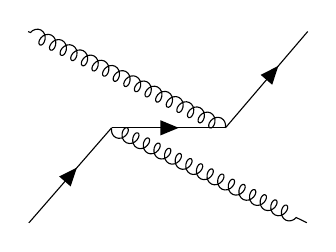
\begin{tikzpicture}[xscale=.95, yscale=1.]
  \begin{feynman}
    \diagram [horizontal=a to b] {
      i1 %[particle=\(Q\)]
      -- [fermion] a
      -- [draw=none] f1,% [particle=\(g\)],
      a -- [fermion] b,
      i2 %[particle=\(Q\)]
      -- [anti fermion] b
      -- [draw=none] f2,% [particle=\(g\)],
    };
    \diagram* {
      (a) -- [gluon] (f2),
      (b) -- [gluon] (f1),
    };
  \end{feynman}
\end{tikzpicture}
\feynmandiagram [xscale=1.2, yscale=.8, horizontal=p2 to p4] {
  p2 [particle=$g$]-- [gluon] b -- [gluon] p4 [particle=$g$],
  a -- [gluon] b,
  p1 [particle=$Q$] -- [fermion] a -- [fermion] p3 [particle=$Q$],
};
\feynmandiagram [xscale=1.2, yscale=.8, horizontal=p1 to p3] {
  p2 [particle=$q$] -- [fermion, edge label=$p_2$] a -- [fermion, edge label=$p_4$] p4 [particle=$q$],
  a -- [gluon, momentum=$q$] b,
  p1 [particle=$Q$] -- [fermion, edge label=$p_1$] b -- [fermion, edge label=$p_3$] p3 [particle=$Q$],
};
\caption{Elastic processes. The first three diagrams contribute to heavy quark (Q) - gluon (g) scattering, the last one contributes to a light (anti-)quark (q) scattering. Intermediate propagators are screened by a Debye mass in case of soft divergence.}\label{plots:feyn-elastic}
\end{figure}

\begin{figure}
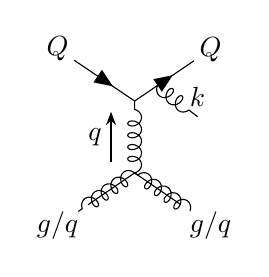
\begin{tikzpicture}
  \begin{feynman}
    \diagram [xscale=0.8, yscale=.6, vertical=a to b] {     
      i2 [particle=\(g/q\)]
        -- [gluon] b
        -- [gluon] f2 [particle=\(g/q\)]],
      b -- [gluon, momentum=$q$] a,
      i1 [particle=\(Q\)]
        -- [fermion] a
        -- [fermion] f1 [particle=\(Q\)],
    };
    \vertex [below right=.2 cm and .8 cm of a, label=\(k\)] (r);
    \draw [gluon] ($(a)!0.3!(f1)$) -- (r);
    \draw  (i2)--(b);
     \draw  (b)--(f2);
  \end{feynman}
\end{tikzpicture}
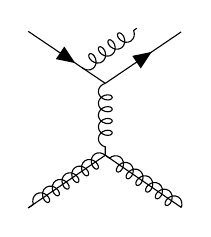
\begin{tikzpicture}
  \begin{feynman}
    \diagram [xscale=0.8, yscale=0.6, vertical=a to b] {     
      i2  -- [gluon] b
        -- [gluon] f2,
      a -- [gluon] b,
      i1 -- [fermion] a
        -- [fermion] f1,
    };
    \vertex [above right=.7 cm and .4 cm of a] (r);
    \draw [gluon] ($(i1)!0.7!(a)$) -- (r);
    \draw  (i2)--(b);
     \draw  (b)--(f2);
  \end{feynman}
\end{tikzpicture}
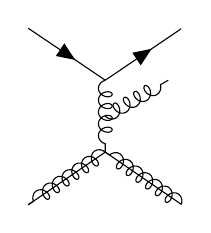
\begin{tikzpicture}
  \begin{feynman}
    \diagram [xscale=0.8, yscale=.6, vertical=a to b] {     
      i2 %[particle=\(g\)]
        -- [gluon] b
        -- [gluon] f2, %[particle=\(g\)]],
      a -- [gluon] b,
      i1 %[particle=\(Q\)]
        -- [fermion] a
        -- [fermion] f1, %[particle=\(Q\)],
    };
    \vertex [below right=.0 cm and .8 cm of a] (r);
    \draw [gluon] ($(a)!0.5!(b)$) -- (r);
    \draw  (i2)--(b);
     \draw  (b)--(f2);
  \end{feynman}
\end{tikzpicture}
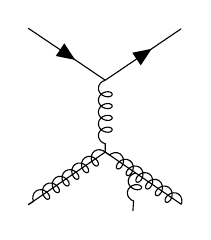
\begin{tikzpicture}
  \begin{feynman}
    \diagram [xscale=0.8, yscale=.6, vertical=a to b] {     
      i2 %[particle=\(g\)]
        -- [gluon] b
        -- [gluon] f2, %[particle=\(g\)]],
      a -- [gluon] b,
      i1 %[particle=\(Q\)]
        -- [fermion] a
        -- [fermion] f1, %[particle=\(Q\)],
    };
    \vertex [below right=.75 cm and .35 cm of b] (r);
    \draw [gluon] ($(i2)!0.6!(b)$) -- (r);
    \draw  (i2)--(b);
     \draw  (b)--(f2);
  \end{feynman}
\end{tikzpicture}
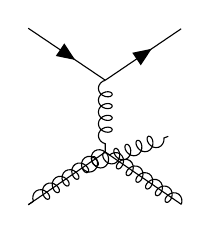
\begin{tikzpicture}
  \begin{feynman}
    \diagram [xscale=0.8, yscale=.6, vertical=a to b] {     
      i2 %[particle=\(g\)]
        -- [gluon] b
        -- [gluon] f2, %[particle=\(g\)]],
      a -- [gluon] b,
      i1 %[particle=\(Q\)]
        -- [fermion] a
        -- [fermion] f1, %[particle=\(Q\)],
    };
    \vertex [above right=.2 cm and .8 cm of b] (r);
    \draw [gluon] ($(b)!0.3!(f2)$) -- (r);
    \draw  (i2)--(b);
     \draw  (b)--(f2);
  \end{feynman}
\end{tikzpicture}
\caption{Inelastic process. Heavy quark collide with a meidum light (anti-)quark or gluon and radiates an additional gluon.}\label{plots:feyn-inelastic}
\end{figure}

\subsection{Diffusion component}
The diffusive motion of heavy quarks between scatterings are solved in Langevin equations in terms of drag and diffusion.
The Langevin equations in the pre-poin Ito scheme are \cite{Rapp:2009my},
\begin{eqnarray}
\Delta \vec{x}_i &=& \frac{\vec{p}_i}{E} \Delta t	\\
\Delta \vec{p}_i &=& -\Gamma \vec{p}_i \Delta t + \Delta t \vec{\xi}(t)
\end{eqnarray}
The first equation is the spatial transport.
In the second equation, momentum of heavy quarks are changed by a drag term with coefficient $\Gamma$ and a thermal random force $\vec{\xi}$. 
The random force has zero mean and the covariance structure:
\begin{eqnarray}
\langle \xi_i \xi_j \rangle = \frac{1}{\Delta t}\left(\Kpara \frac{p_i p_j}{p^2} + \Kperp \left(\delta_{ij} - \frac{p_i p_j}{p^2}\right) \right)
\end{eqnarray}
In this study, we assume an isotropic diffusion component $\Kpara=\Kperp=\kappa$.
The drag coefficient $\Gamma$ and the momentum diffusion coefficient $\kappa$ need to satisfy the Einstein relation in pre-point Ito scheme to guarantee the approach of the correct thermal equilibrium \cite{Rapp:2009my},
\begin{eqnarray}
\Gamma &=& \frac{\kappa}{2TE} - \frac{d\kappa}{dp^2}
\end{eqnarray}
We choose to parametrize the momentum diffusion constant $\kappa$ and the drag is determined as above.
If temperature is the only scale in the problem, we expect $\kappa$ to scale as $T^3$.
Additional, we consider the possibility of non-perturbative contribution to the diffusion component, which may be strong at low energy and low temperature and we arrive at the following simple ansatz,
\begin{eqnarray}
\frac{\kappa}{T^3} = \kappa_D\left(x_D + (1-x_D)\frac{\textrm{ GeV}^2}{ET}\right)
\end{eqnarray}
$\kappa_D$ is the strength of diffusion at $ET = 1\textrm{ GeV}^2$, and $x_D$ interpolates between the two types of energy-temperature dependence.

\section{Tests in a static medium}\label{section:test}
\begin{figure}
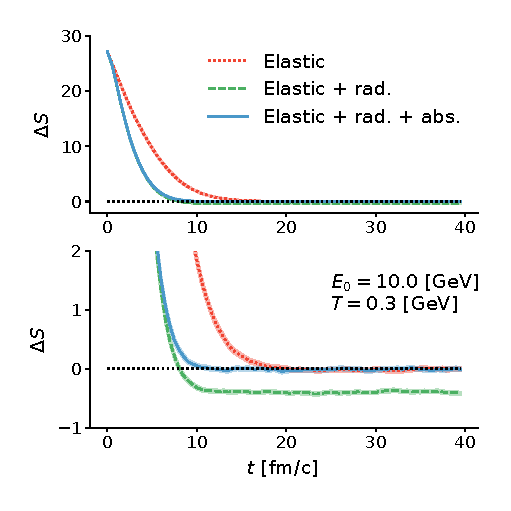
\includegraphics[width=\columnwidth]{thermalization.pdf}
\caption{The approach to thermalization of the linear Boltzmann equation with elastic processes only (red dot), elastic with radiation processes (green dashed), and elastic with both radaition and absorption processes (blue solid). The static medium has a temperature $T = 0.4$ GeV. $10^4$ heavy quarks are initialized with $E = 10$ GeV at $t = 0$.}\label{plots:thermalization}
\end{figure}

Before coupling the heavy quark transport model to a realistic medium, we study the model in a static medium, i.e., the medium is at rest with a fixed temperature.
All the calculation in this section uses $\mu =1$.

A first test is to check our implementation indeed respect detailed balance and reaches the thermal equilibrium.
To quantify the approaching to the thermal distribution of an ensemble of $N$ heavy quarks in a medium with temperature $T_0$, we define the following indicator $\Delta S$,
\begin{eqnarray}
\Delta S = \frac{1}{N}\sum_{i=1}^{N} \ln f_0(E_i) - \frac{\int f_0(p)\ln f_0(E) dp^3}{\int f_0(p) dp^3}
\end{eqnarray}
$f_0 \propto \exp(-E/T_0)$ is the Boltzmann-J\"uttner distribution function at temperature $T_0$. 
The first term takes the heavy quarks ensemble average of $\ln f_0(E)$ and the second term is proportional to the entropy at $T_0$,
This difference $\Delta S$ defines a ``distance" from the heavy quark ensemble to the thermal distribution, and it vanishes when the ensemble thermalizes.
If the ensemble distribution function $f$ is not far from equilibrium and can be characterized by an effective temperature $T_{\textrm{eff}}$ so that $f(E)\sim \exp(-E/T_{\textrm{eff}})$, then this ``distance" measures,
\begin{eqnarray}
\nonumber
\Delta S &\sim& \frac{1}{T_0}\int  e^{-E/T_{\textrm{eff}}} E dp^3 - \frac{1}{T_0}\int e^{-E/T_0} E dp^3 \\
&=& \frac{T_\textrm{eff}-T_0}{T_0},
\end{eqnarray}
which is the fractional deviation of the effective temperature from the temperature of the thermal bath.
Figure \ref{plots:thermalization} shows the time-evolution of $\Delta S$ of $10^4$ charm quarks inside thermal bath $T=0.4$ GeV with initial energy $E_0 = 10$ GeV.
With elastic process only, the system thermalizes after about $50$ fm/$c$.
If we further turn on radiation process, the system reaches equilibrium faster, but it is wrong equilibrium.
The effective temperature is lower than the temperature of the thermal bath $T_0$.
This is the consequence of breaking detailed balance without the reverse process of radiation.
Finally, we showed the case with both radiation and absorption turned on, the correct equilibrium is reached at $t\sim 20$ fm/c.
The absorption processes only make a notable difference when the system is not far from equilibrium ($\Delta S < 1$), which is expected from our previous argument.
\begin{figure}
\includegraphics[width=\columnwidth]{Eloss.pdf}
\caption{Top row: energy loss fraction as function of energy for elastic processes (left) and ineasltic processes (right). Bottom row: energy loss fraction as function of path length for elastic processes (left) and ineasltic processes (right).}\label{plots:dEE}
\end{figure}
\begin{figure}
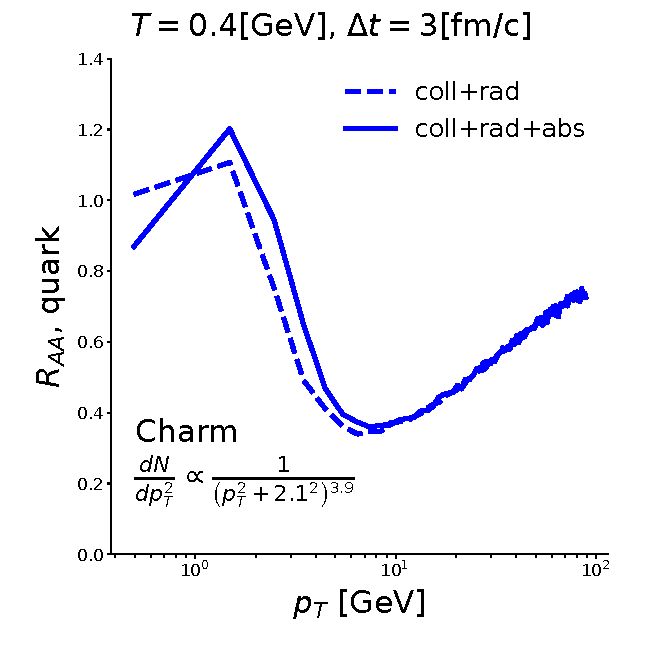
\includegraphics[width=\columnwidth]{BoxRaa.pdf}
\caption{$R_{AA}$ in a static medium for charm and bottom. The medium size  is $3$ fm and has a temperture $T_0 = 300$ MeV. The initial spectra of charm and bottom is a simple power law form with fit from \cite{Cao:2012jt}.}\label{plots:BoxRaa}
\end{figure}

Next we study the heavy quark energy loss in a static medium.
Na\"ively, energy loss per unit time can be calculated by inserting $\Delta E$ into the integration of the rate equation \ref{eq:rate}. 
This is straightforward for elastic processes, but because the rates of inelastic processes depend on history, so a meaningful energy loss can only result from an actually Monte Carlo simulation.
And as we will see, this history dependence causes a non-trivial path length (medium size $L$) dependent energy loss.
In the first row of Figure \ref{plots:dEE}, we plot energy loss fraction $\Delta E/E$ for elastic process (left) and inelastic process (right) as function of $E$ for path length $5$ fm and temperature $T=0.2$ and $0.4$  GeV.
The elastic energy loss fraction is large at intermediate energy and decreases towards small and large energies.
At sufficient low energy, heavy quarks starts to gain energy from the medium on average that manifests as $\Delta E/E < 0$.
For the case of inelastic energy loss, we study the effect of gluon absorption process by comparing $\Delta E/E$ with only radiation process (lines) to $\Delta E/E$ with both gluon radiation and absorption (lines with symbols).
As expected, we find that gluon absorption process only affects energy loss significantly for low ratio of $E/T$.
At sufficient low energy, gluon absorption process allow the heavy quark to gain energy from the medium through inelastic channel which is key to thermalization.
In the second row of Figure \ref{plots:dEE}, we show the path length dependence of the two energy loss mechanism.
Here, we plot the energy loss fraction per unit length, with length measured in units of inverse temperature.
The key observation is that elastic energy loss increases linearly with path length but inelastic energy loss increases non-linearly for small path length and then transits to a linear increase at large path length. 
The non-linear $L-$dependence is a characteristic behavior of the coherence effect in a finite length medium. 
In our effective LPM implementation, this arises because the gluon radiation with $\tau_f \sim k/T^2 \gg L$ is suppressed.
Therefore for a thin medium, the phase space for gluon radiation is very restricted $k < LT^2$, and this is also the typical amount of energy loss per radiation.
Multiplying $k \sim LT^2$ by the number of collisions $N \propto LT$, the inelastic energy loss scales as $\Delta E \sim L^2T^3$.
For a thick medium, a heavy quark could have multiple radiations with $N \propto L/\tau_f$ and each radiation carries off a typical amount of energy. 
In this region, the inelastic energy loss rises linearly with $L$.
What we see in the simulation is a behavior that interpolates between these two qualitative behaviors.

Finally, we calculate the $R_{AA}$ of charm and bottom quark in a static medium $T=0.4$ GeV after evolving for $3$ fm/c.
The initial spectra of the charm and bottom are parametrized in a simple power law form \cite{Cao:2012jt}.
This simplified setup is intended for comparison with other models with controlled settings.
In Figure \ref{plots:BoxRaa} we showed both $R_{AA}$ of charm and bottom with or without the gluon absorption process. 
Again, we see that the absorption process only affects observables for relatively low momentum $p_T < 10$ GeV.
The mass plays an important role in the intermediate $p_T$ region, where a clear separation between charm and bottom $R_{AA}$.
The mass effect is neither important at high energy where $p_T$ is the only relevant scale or low $p_T$ when $M (\gg p_T, T)$ becomes the only relevant scale. 

\section{Calibration of the model at LHC using Bayesian analysis}\label{section:calibration}
In this section, we couple the heavy quark transport model to the state-of-the-art 2+1D event-by-event medium evolution and extract the transport model parameters from a Bayesian model-to-data comparison.
The medium evolution model consists of multiple stages,
\begin{itemize}
\item[1.] The TRENTo model generates event-by-event initial condition at time $\tau = 0^+$ \cite{Moreland:2014oya}. 
\item[2.] A collision-less Boltzmann equation (freestreaming) models the pre-equilibrium stage before the start of hydrodynamics expansion at $\tau_{fs}$ \cite{Liu:2015nwa}.
\item[3.] The 2+1D relativistic viscous hydrodynamics evolves the QGP with an up-to-date lattice equation of state \cite{Shen:2014vra, Bazavov:2014pvz}.
\item[4.] Finally, hadrons sampled from hydrodynamic energy momentum tensors rescatter and decay in the Ultra-Relativistic Quantum Molecular Dynamics (UrQMD) model \cite{Bass:1998ca, Bleicher:1999xi}.
\end{itemize}
The parameters of this bulk event generator have already been calibrated to reproduce a vast of bulk observables at the LHC energies [Jonah's analysis with freestreaming is not public yet], providing a description of bulk evolution with unprecedented precision.
On the heavy quark transport side, we initialize heavy quark ensembles with the momenta sampled from FONLL calculation using two different sets of nuclear parton distribution function \cite{Cacciari:1998it,Kovarik:2015cma,Eskola:2016oht}. 
The nuclear PDF comes with large uncertainty in the shadowing region which is relevant at the LHC energies.
It is hard to systematically include its uncertainty in our study; instead, we choose to use the center values of two different sets of nuclear PDF, namely the EPPS set and the nCTEQ16np set and perform calibrations using both to demonstrate the sensitivity of the parameter extraction on the nuclear PDF uncertainty.
The difference between the two can to some extent reflects the uncertainties in our understanding of the nuclear shadowing effects.
The position of the hard production vertices at $\tau = 0^+$ are sampled from TRENTo binary collision density to correlate with hot-spots of  underlying event. 
During the pre-equilibrium stage the heavy quark should already start to interact with medium.
The system at this stage is still far from both kinetic and chemical equilibrium.
To get a handle on the effect of pre-equilibrium energy loss, we choose to define the medium flow velocities and energy density from the pre-equilibrium energy-momentum tensor by Landau matching and further convert the energy density to a temperature using a 3-flavor conformal QCD equation of state. 
Heavy quarks are allowed to loose energy starting from a tunable energy-loss starting time $0.1\textrm{ fm/c} < \tau_0 < \tau_{\textrm{fs}}$. 
With a small $\tau_0$, this correspond to a fast generate of degrees of freedom in the medium that can collide with heavy quarks at very early time, and with a large $\tau_0$ the pre-equilibrium effects gradually turns off.
This is of course a very crude setup and we are looking for more sophisticated models to treat pre-equilibrium stage energy loss such as a parton cascade model \cite{Srivastava:2017bcm}.
During the hydrodynamic expansion stage, the time evolution of the flow velocities and temperature are provided by the 2+1D viscous hydro dynamics with boost-invariance in the beam direction.
The heavy quarks then hadronize in a sudden-approximation at $T = 154$ MeV through both the fragmentation and recombination mechanisms \cite{Cao:2013ita}. 
The bottomed mesons cease to interact at this point in our model, but the charmed mesons are included in the UrQMD afterburner with $\pi$-D and $\rho$-D cross-sections \cite{Lin:2000jp}.

The free parameters in the heavy flavor sector simulation are,
\begin{itemize}
\item[1.] $\tau_0$ the time at which heavy quark energy loss starts, varies between $0.1$ fm/c to $1.0$ fm/c.
\item[2.] $\mu$, the medium energy scale ($\mu\pi T$) parameter that appears in the running coupling constant of the scattering component, varies from $1/3$ to $4$.
\item[3.] $\kappa_D$, the strength of momentum diffusion at $ET = 1 \textrm{GeV}^2$, range from $0$ to $8$.
\item[4.] $x_D$, the fraction of the momentum diffusion that is energy independent, ranges from $0$ to $1$.
\end{itemize}
In additional to these continuous parameters, the choose of different nuclear parton distribution function as a discrete variable.

Here, we briefly introduce the idea of this Bayesian technique and key terminologies to be used later.
For more details, one can refers to the thesis work \cite{Bernhard:2018hnz} for an exhaustive study and to previous works for applications to bulk evolution \cite{Bernhard:2015hxa,Bernhard:2016tnd} and to heavy quark sector with an improved Langevin transport model \cite{Xu:2017obm}.
Given a model whose prediction ${\bf y}$ depends on a vector of input parameters ${\bf p}$ and the experimental data ${\bf y}_\textrm{exp}$, 
the probability distribution of the {\it true} model parameters ${\bf p^*}$ is given by the Baye's theorem, 
\begin{eqnarray}\label{eq:Bayes}
\textrm{Posterior}({\bf p^*}|{\bf y}_\textrm{exp}, M) &\propto& \textrm{Likelihood}({\bf y}_\textrm{exp}|{\bf p^*}, M) \nonumber \\ &\times& \textrm{Prior}({\bf p^*}).
\end{eqnarray}
The posterior probability distribution of the ${\bf p^*}$ given certain model $M$ and data, equals the probability $L$ of observing data given model and parameters ${\bf p^*}$, called likelihood function, times a prior belief on the distribution of ${\bf p^*}$.
The likelihood function is often defined in a Gaussian form in terms of the difference between model calculation and experimental data and a covariance matrix $\Sigma$ that encodes experimental and theory uncertainty,
\begin{eqnarray}\label{eq:likelihood}
\ln(L) &=& -\frac{1}{2}({\bf y}-{\bf y}_{\textrm{exp}})^T\Sigma^{-1} ({\bf y}-{\bf y}_{\textrm{exp}})\nonumber\\ 
		&-&\frac{d}{2}\ln(2\pi)-\frac{1}{2}\ln|\Sigma|.
\end{eqnarray}
The construction of $\Sigma$ is described in Appendix \ref{appendix:sigma}
Once we have the ability to evaluate model output given arbitrary parameters within a reasonable range, the information of parameters constrained by data follows from Equations \ref{eq:Bayes} and \ref{eq:likelihood}.
And this high-dimensional posterior probability distribution function can be studied by a Markov-chain Monte Carlo (MCMC) sampling procedure.
The difficulties for applying this directly event-by-event heavy-ion collision simulation are that the model itself is computationally expensive and that $\mathcal{O}(10^4)$ minimum-biased events are needed to get statistical error of the simulation under control.
Therefore, it is unpractical to evaluate the model output at arbitrary points in the parameter space in during the MCMC sampling.
The solution is to use advanced sampling technique and only evaluate the full model at $\mathcal{O}(100)$ design parameter sets (design points).
Then, the model outputs at arbitrary point in the parameter space are fast interpolated by a Gaussian process emulator that has trained on the full model calculation at design points \cite{Rasmussen:2006gp}.
\begin{center}
\begin{table}[h]
\caption{ALICE dataset}\label{table:ALICE-obs} 
\begin{tabularx}{\columnwidth}{XXX}
\hline 
 Observables & Centrality & Reference\\ 
\hline 
D-meson $v_2$ & 30-50\% & \cite{Acharya:2017qps}\\ 
\hline 
Event-engineered D-meson $v_2$ & 30-50\% & \cite{Grosa:2017zcz}\\ 
\hline 
D-meson $R_{AA}$ & 0-10, 30-50, 50-80\% & \cite{Acharya:2018hre}\\
\hline 
\end{tabularx}
\end{table}
\begin{table}[h]
\caption{CMS dataset}\label{table:CMS-obs} 
\begin{tabularx}{\columnwidth}{XXX}
\hline 
Observables & Centrality & Reference\\ 
\hline 
D${}^0$-meson $v_2$ & 0-10, 10-30, 30-50\% & \cite{Sirunyan:2017plt}\\ 
\hline 
D${}^0$-meson $R_{AA}$ & 0-10\%, 0-100\% & \cite{Sirunyan:2017xss}\\ 
\hline 
B${}^{\pm}$-meson $R_{AA}$ & 0-100\% & \cite{Sirunyan:2017oug}\\ 
\hline 
\end{tabularx}
\end{table}
\end{center}

In this work, we sampled 80 design points in the four dimensional parameter space $(\tau_0, \mu, \kappa_D, x_D)$.
For each parameter set, we ran 4000 minimum biased events.
Each event propagates an ensemble of $4\times 10^4$ charm quarks and $10^4$ bottom quarks.
The centrality is defined by mid-rapidity charged particle multiplicity and the same kinematic cuts as experimental measures are applied to the calculation of heavy flavor observables.
All these observables are measured at 5.02 TeV in Pb+Pb, as listed in Table \ref{table:ALICE-obs} and \ref{table:CMS-obs} and here are a few remarks on our choice.
Most of these data are for D-meson.
There are $p_T$ dependent D-meson nuclear modification factor $R_{AA}$ and $p_T$ dependent second-order azimuthal anisotropy $v_2$ at various centralities \cite{Sirunyan:2017plt, Sirunyan:2017xss, Acharya:2017qps,Grosa:2017zcz}.
We also compare to the event-engineered D-meson flow being measured at ALICE \cite{Grosa:2017zcz}.
The idea of the event-engineering is to subdivide events in a certain centrality according to the magnitude of charged particle $q$-vector, in this case,
\begin{eqnarray}
|q_2|^2 = \frac{\left(\sum_{i=1}^{M} \cos(2\phi) \right)^2+ \left(\sum_{i=1}^{M} \sin(2\phi) \right)^2}{M}
\end{eqnarray}.
The D-meson $v_2$ is measured for those events with $20\%$ highest $q_2$ and events with $60\%$ lowest $q_2$.
It is found that D-meson flow is strongly correlated with this measure of bulk collectivity.
This event-engineering procedure necessitates a full event-by-event study and may be sensitive to the interplay between heavy quark energy loss and initial condition fluctuation, so we include into the set of observables on which we calibrate the model.
Finally to require the calibrated model predicts the desired mass-dependence, we include recent CMS measurements of $B^{\pm}$-meson $R_{AA}$, although the data has a large uncertainty which decreases its importance in the likelihood function.
\begin{figure*}
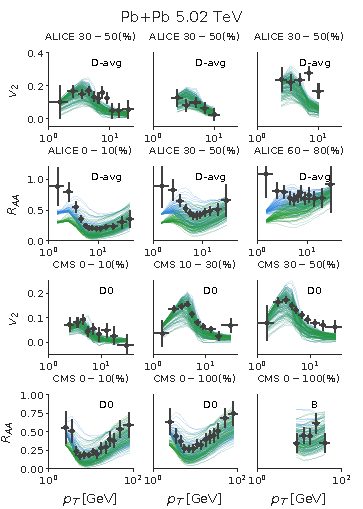
\includegraphics[width=.49\textwidth]{observables_design.pdf}
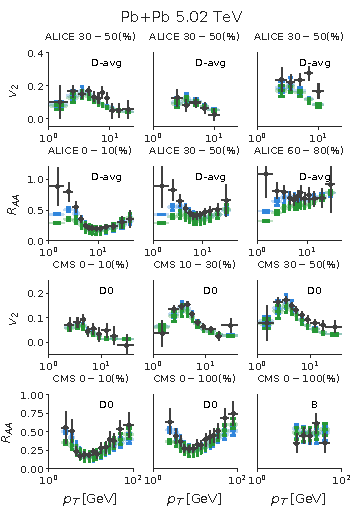
\includegraphics[width=.49\textwidth]{observables_posterior.pdf}
\caption{Left: prior range of model calculations. Right: posterior observables from model emulators. In both figures, blue(green) lines are calcualtions with EPPS (nCTEQ15np) nuclear PDF}\label{plots:deisgn_posterior_obs}
\end{figure*}

On the left of Figure \ref{plots:deisgn_posterior_obs}, we show the prior range of our calculations for each of the listed observables. 
We use different colors to distinguish calculations using EPPS (blue) and
nCTEQnp (green) nuclear PDF.
The calculated $R_{AA}$ at high transverse momenta and $v_2$ at low transverse momenta are spread enough to cover the experimental data.
We noticed that the model always underestimates the very low-$p_T$ $R_{AA}$ and 30-50\% high-$p_T$ $v_2$ from CMS.
This could be limitations of our model, such as the need of more sophisticated implementation of LPM effect and more accurate calculation of low-$p_T$ charm quark production in both $p-p$ and $A-A$ collisions. 
Plots on the right of Figure \ref{plots:deisgn_posterior_obs} show the posterior distribution of the observables from model emulators.
The calibrated model displays a very good overall fit to all the observables except for the limitations pointed out above.
The use of different nuclear PDF makes negligible difference for azimuthal anisotropy, but does affect the $R_{AA}$ at small and large $p_T$.
Calculations with EPPS nuclear PDF works very well in describing $R_{AA}$ below $p_T = 50$ GeV, while calculations with nCTEQnp does slightly better for CMS $R_{AA}$ with $p_T>50$ GeV.
The calculated event-engineered flow strongly correlates with the charged particle $|q_2|$ and describes the lowest 60\% $q_2$ bin very well.
For the highest 20\% $q_2$ bin, model posterior is consistent with measurements below $5$ GeV and underestimates the data at higher $p_T$ bins.

\begin{figure}
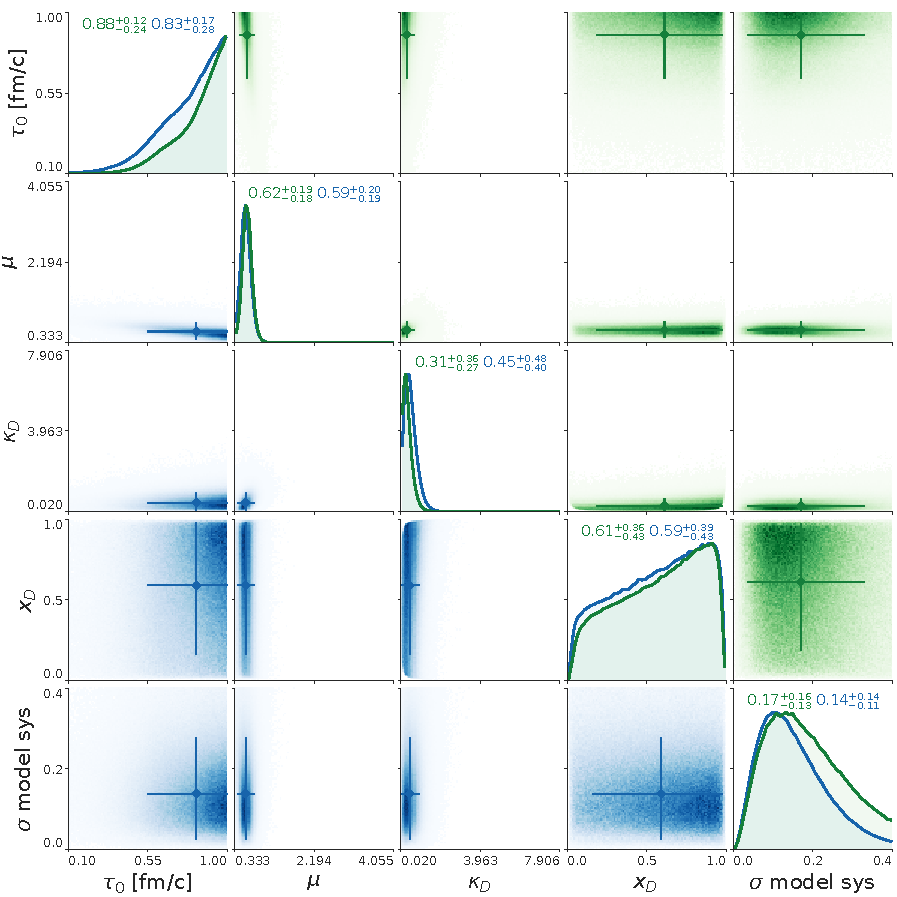
\includegraphics[width=.5\textwidth]{posterior.pdf}
\caption{Marginalized postrior probability distribution of model parameters. Dignoal plots show the marginalization on a single parameters. Off diagonal plots show the pair correlation between parameters. Blue (Geen) lines and lower (upper) off diagnoal plots corresponds to the extraction using EPPS (nCTEQ15np) nuclear PDF}\label{plots:posterior}
\end{figure}
\begin{figure}
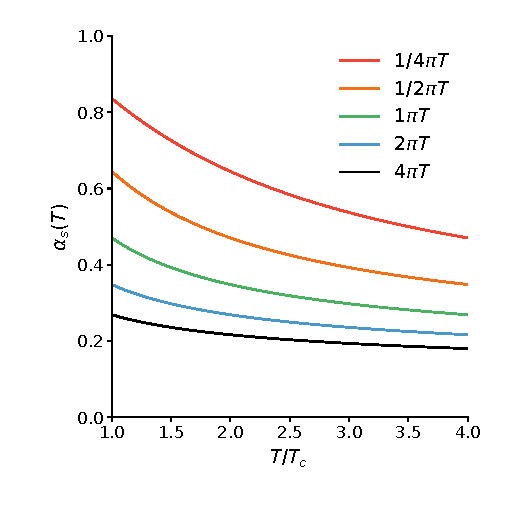
\includegraphics[width=.5\textwidth]{alpha_s_at_T.pdf}
\caption{Coupling constant with three values of medium scale parameter $\mu$ that comes from the high likilihood region of the posterior. Left: evaluate $\alpha_s$ at process scale $Q=0$. Right: evaluate $\alpha_s$ at process scale $Q=m_D$.}\label{plots:alphas}
\end{figure}

The posterior probability distribution of the parameters are marginalized to single parameter distribution (diagonal) and two-parameter joint distribution (off-diagonal) in Figure \ref{plots:posterior}.
The lower off-diagonal plots and blue lines in the diagonal plots correspond to the extraction using EPPS nuclear PDF, and the off-diagonal plots and green lines in the diagonal plots uses nCTEQ15np nuclear PDF.
Despite the difference in $R_{AA}$ when different nuclear PDFs are used, the extracted probability distribution of parameters are similar.
To describe LHC data, the model prefers a late onset of medium induced energy loss and a medium energy scale roughly around $0.6\pi T$, which means the largest coupling constant at certain temperature is $\alpha_s \sim \alpha_s(1.8T)$.
A small but finite amount of momentum diffusion at $ET=1\textrm{ GeV}^2$ is preferred for the diffusion component.
The smallness of this number is expected because most of the interaction are already taken account by the scattering component with relatively large coupling constant (a small medium scale).
But this study is not sensitive to the energy / temperature dependence of the diffusion component other than the regular $T^3$ scaling of the momentum diffusion constant.   

We notice that the preferred medium scale that acts as a minimum energy scale cut-off in $\alpha_s(Q, \mu\pi T)$ is not very large.
So it is imperative to check the typical $\alpha_s$ in the model to evaluate the the use of perturbative matrix-elements.
Here we evaluate the strong coupling constant at two process scales $Q=0$ and $Q=m_D$ in Figure \ref{plots:alphas}.
In the case of $Q=0$ (left), the energy scale is cut off by $\mu\pi T$ and this plot show the maximum of model coupling constant at a given temperature.
Put $Q=m_D$ (right) as a proxy for the typical momentum transfer in the $t-$channel scattering, the coupling constant rises slower as temperature drops down.
It turns out in order to describe experimental data, the preferred coupling constant is fairly large suggesting next-to-leading (NLO) order correction to the present scattering picture should be prominent.
One may even question the use of a perturbative expansion with such large coupling.
It would be interesting to study if a calibration with NLO level processes would result in a better control of the coupling constant in the medium.

Next, we investigate the transport coefficients of the calibrated model.
To define the total momentum broadening parameter of a heavy quark,
we combine the contribution from both elastic scatterings and the diffusion component,
\begin{eqnarray}\label{eq:qhat}
\frac{\hat{q}}{T^3} &=& \frac{1}{T^3}\frac{d}{dt}\left\langle p_\perp^2 \right\rangle\\
\nonumber
 &=&  \kappa_D\left(x_D + (1-x_D)\frac{\textrm{GeV}^2}{ET}\right) + \frac{\hat{q}_{\textrm{el}}}{T^3}.
\end{eqnarray}
Where $\hat{q}_{\textrm{el}}$ is obtained by integrating the rate equation with transverse momentum transfer square.
We shall discuss the inclusion of inelastic process into the calculation $\hat{q}$ in section \ref{section:conclusion}.
Performing this calculation for many random parameter set samples drawn from the posterior distribution using either nuclear PDF, we estimate the posterior distribution of the functional $\hat{q}(E, T)$ constrained by data.
On the left of Figure \ref{plots:posterior_qhat}, we showed the 90\% credible region of $\hat{q}$ as function of temperature, fixing heavy quark momenta at $10$ GeV.
And the right panel the figure shows $\hat{q}$ as function of momenta at $T=0.35$ GeV.
Our formula is mass dependence and the charm quark $\hat{q}$ (region enclosed by thick red lines and slashes) is slightly different from the bottom quark $\hat{q}$ (region enclosed by thick blue lines).
Comparing to former work by Yingru et al (shaded region), who used an improved Langevin model to extract charm quark transport properties at the LHC, the present result is consistent but hits the lower half of the 90\% credible region of the previous extraction.
\begin{figure}
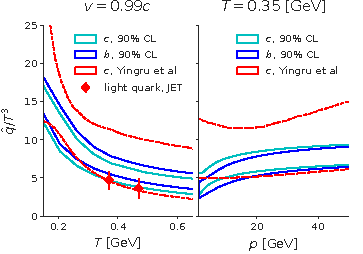
\includegraphics[width=\columnwidth]{qhat_p_T.pdf}
\caption{Posterior range of heavy quark transverse momentum broadening parameter $\hat{q}$ from Equation \ref{eq:qhat}. The results already include uncertainty from using different nuclear PDF. Blue boxed region are for bottom quark and red slahed region for charm quark. The shade region indicates previous extraction \cite{Xu:2017obm}.}\label{plots:posterior_qhat}
\end{figure}
There is also a heavy quark spatial diffusion constant $D_s$ often defined in the limit of $p\ll M$.
It is related to the momentum diffusion parameter by,
\begin{eqnarray}
2\pi T D_s = \frac{8\pi T^3}{\hat{q}(p\rightarrow 0, T)}
\end{eqnarray}
In figure \ref{plots:posterior_Ds}, we plotted the 90\% credible region of both charm (region enclosed by red thick lines and slashes) and bottom (region enclosed by blue tick lines) quark spatial diffusion constant as function of $T/T_c$.
The results of this work is systematically higher than the extraction from the former work (shaded region).
The spatial diffusion constant has been calculated from first principal using lattice QCD.
There are two calculations available, one in the static heavy quark limit (blue symbols with higher values and larger errorbars) and the other for realistic charm quark (red symbols with lower values and smaller errorbars).
Our posterior in $D_s$ with diffusion component and only elastic channel contribution agrees with the static heavy quark limit lattice evaluation.
The effect of including inelastic channel in $D_s$ is discussed in the last section.

To summarize this section, we performed a Bayesian calibration on the model parameters. 
We find a general agreement to the data.
Although the use of different nuclear shadowing parametrization do affect the shape of $R_{AA}$, the extracted parameters posterior probability distribution is not strongly affected.
The extracted parameters indicate a late onset of medium induced heavy quark energy loss and a small by finite diffusion component is preferred.
The posterior transport coefficient $\hat{q}$ and spatial diffusion constant $D_s$ is calculated and $D_s$ agrees with lattice calculation in the static heavy quark limit. 

\begin{figure}
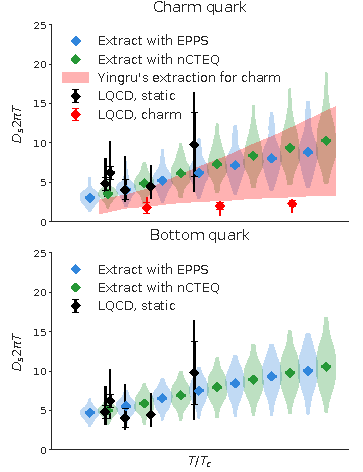
\includegraphics[width=\columnwidth]{Ds_posterior.pdf}
\caption{Posterior range of heavy quark spatial diffusion coefficient. Blue boxed region are for bottom quark and red slahed region for charm quark. The shade region indicates previous extraction in \cite{Xu:2017obm}. Symbols with larger errorbars are lattice evaluation for static heavy quark and symbols with smaller errorbars are lattice evaluation for dynamic charm quark.}\label{plots:posterior_Ds}
\end{figure}

\section{Validation and Prediction}\label{section:prediction}
We now apply the calibrated model to calculate observables that has already been measured but excluded in the calibration (validation) and also predict novel observables.
In principal, any parameter sets sampled according to the posterior probability distribution in the high-likelihood region (90\% credible for example) are equally good to make predictions and the resultant differences represent the systematic uncertainties of the prediction.
For simplicity, we only run a single set of high likelihood parameters listed in Table \ref{table:high-likelihood-parameters} with very high statistics.
\begin{table}
\caption{A high-likelihood parameter set}\label{table:high-likelihood-parameters}
\begin{tabularx}{\columnwidth}{XXXXX}
\hline
Parameters & $\tau_0$ [fm/c] & $\mu$ & $\kappa_D$ & $x_D$   \\
\hline
Values & 0.9 & 0.6 & 0.4 & 0.5\\
\hline
\end{tabularx}
\end{table} 
\begin{figure*}
\includegraphics[width=\textwidth]{raa.pdf}
\caption{Calculation of heavy-flavor $R_{AA}$ with the high likelihood parameter set compared to ALICE D-meson Pb+Pb and p+Pb \cite{Abelev:2014hha} measurements. B-meson $R_{AA}$ are predictions.}\label{plots:pred:raa}
\end{figure*}
\begin{figure*}
\includegraphics[width=\textwidth]{vn.pdf}
\caption{Calculation of heavy-flavor flows with the high likelihood parameter set compared to CMS D-meson measurements. D-meson $v_3$ and B-meson $v_2, v_3$ are predictions.}\label{plots:pred:vn}
\end{figure*}
\begin{figure}
\includegraphics[width=0.5\textwidth]{v1.pdf}\\
\includegraphics[width=0.5\textwidth]{v1pT.pdf}
\caption{Top row: centrality dependence of D-meson direct flow with respect to $n=3$ event plane. Left: the prior range. Right: prediction using high likelihood parameter set. Bottom left: the transverse momentum dependence of D-meson direct flow with respect to $n=3$ event plane at 30-50\% centrality. Bottom right: a sample trento event. The third order eccentricity would drive a $v_3$. A measurement along the $n=3$ direction, would introduce reflection asymmetry in the heavy quark energy loss.}\label{plots:pred:v1}
\end{figure}
We first investigate the B-meson nuclear modification factor in a larger $p_T$ range with ALICE kinematic cuts.
In Figure \ref{plots:pred:raa}, B-meson $R_{AA}$ for 0-10\%, 30-50\%, and 60-80\% centrality is shown and compared to D-meson calculations and measurements for a reference.
The mass effect clearly separates B-meson from D-meson $R_{AA}$ in the intermediate $p_T$ range for all three centralities. 
CMS has measured the third harmonics flow of D-meson, showing a non-zero $v_3$ at relatively low transverse momentum that weakly dependents on centrality.
In the transport model, non-zero heavy-flavor $v_3$ is caused by heavy quarks losing energy to a medium with third order eccentricity from initial condition fluctuations.
The fluctuation nature of $v_3$ requires averaging over much more events than the calculation of $v_2$ to control the statistical fluctuation and as a result we did not include it in the calibration.
We validate our calibration with the D-meson $v_3$ and make a prediction for B-meson $v_n$ in Figure \ref{plots:pred:vn}.
The B-meson $v_2$ and $v_3$ is predicted to be similar to D-meson flow for $p_T > 10$ GeV, below which B-meson flow is significantly smaller than D-meson flow.
Compared to CMS data, the calibrated model reproduces the transverse momentum and centrality dependence of D-meson $v_3$ very well.

Finally, we want to bring attention to the D-meson direct flow $v_1$.
D-meson $v_1$ should be vanishing at mid-rapidity if one measures it with respect to an estimation of reaction plane due to the reflection symmetry on averaging over many events.
But we can correlate heavy quarks $v_1$ with charged particle $v_3$ to get a non-zero signal even at mid-rapidity.
This direct flow with respect to $n=3$ event plane is calculated in the scalar product approach
\begin{eqnarray}
v_1 &=& \left\langle \frac{\Re\{q_3 Q_1^*\}}{mM} \right\rangle\Bigm/\left\langle \frac{|q_3|^2-m}{m(m-1)} \right\rangle,\\
Q_1 &=& \sum_{j=1}^{M}e^{i\phi_j} \textrm{, for heavy mesons},\nonumber\\
q_3 &=& \sum_{j=1}^{m}e^{i3\phi_j} \textrm{, for charged particles}. \nonumber
\end{eqnarray}
The resulting $v_1$ as function of centrality is shown in Figure \ref{plots:pred:v1}.
The shaded area is the prior range of this quantity using events from the 80 design parameter set calculations.
The dots are our prediction using the high likelihood parameter set with ALICE kinematic cuts.
This quantity is clearly finite and negative in our calculation and we expect it to reach as far as $-4\%$ in the peripheral centrality bin.
We understand this finite signal in the following way. 
When $q_3$ is finite, the direction of $q_3$ defines a plane to which the medium evolution is reflection asymmetric and this asymmetry causes heavy quarks to loose energy differently depending whether the direction of motion is along or against the direction of $q_3$.
Since $q_3$ originates from the triangular initial state fluctuation, a finite signal would be another indication of heavy quark energy loss coupling to initial condition fluctuations and bulk collectivity.

\section{Discussion and Conclusion}\label{section:conclusion}
\begin{figure}
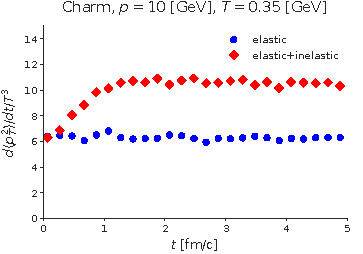
\includegraphics[width=0.5\textwidth]{qhat_full.pdf}
\caption{Comparing heavy quark transport coefficient (left: $\hat{q}$, right $D_s$) with (solid lines) and without (dashed lines) including inelatic contribution. Thin blue lines are for bottom quark and thick red lines region charm quark. Symbols with larger errorbars are lattice evaluation for static heavy quark and symbols with smaller errorbars are lattice evaluation for dynamic charm quark.}\label{plots:transport_full}
\end{figure}
Before summarizing this work, we want to discuss more on the definition of $\hat{q}$ in our model.
In Equation \ref{eq:qhat}, we used only the elastic processes in the second term and did not include inelastic contribution to momentum broadening.
This is because we have an order-by-order definition of $\hat{q}$ in pQCD.
In fact, the inelastic processes also contributes a diffusion-like part, but is shown to be one order higher in $\alpha_s$ \cite{Ghiglieri:2015ala}, though it may not be numerically small in realistic case compared to leading order.
So in the sense of calculating a leading order transport coefficient we justify the use of Equation \ref{eq:qhat}. 
This choice is also conceptually cleaner to compare with other pQCD based calculations.
For lattice calculations the results do not rely on an expansion in $\alpha_s$.
In that case, to make a reasonable comparison with lattice transport coefficients, we should calculate $\hat{q}$ from the calibrated model including the inelastic processes.
Unfortunately, currently there is not any lattice calculation of $\hat{q}$ at finite heavy quark momenta.  
$D_s$ on Lattice do exist, but such momenta ($p \ll M$) are too small for our calculation with Gunion-Bertsch matrix-elements to be valid.
Even so, we would like to show the $\hat{q}$ and $D_s$ with a set of high likelihood parameters that includes the inelastic contribution.
Just like the energy loss showed in Figure \ref{plots:dEE}, the transverse momentum broadening per unit time in the presence of inelastic processes is not a constant for a thin medium.
Therefore, we setup the Monte Carlo simulation for fixed energy heavy quarks and extract $\hat{q}$ only after the finite path length effect fades away. 
Figure \ref{plots:transport_full} compares the $\hat{q}$ at $p=10$ GeV and $D_s$ with and without inelastic channels.
The calculation uses the high likelihood parameter set in Table \ref{table:high-likelihood-parameters}. 
We observe a 30-40\% increase in $\hat{q}$ and similar amount of decrease in $D_s$ with the inelastic contribution.

In conclusion, in this work we developed a linearized hybrid transport model for heavy quark propagation inside a quark-gluon plasma.
Heavy quark undergoes perturbative scatterings with medium particles. Between subsequent scatterings, the propagation are driven by Langevin dynamics with empirical drag and diffusion constant.
Model parameters are calibrated using Bayesian technique by comparing to D -meson and B-meson observables in Pb+Pb collisions at $\sqrt{s}=5.02$ TeV.
Our results suggest a late onset of medium energy loss.
The typical coupling constant of perturbative scattering is fairly large and future improvements are needed.
A additional small diffusion component is preferred.
The calibrated model predicts the centrality and $p_T$ dependence of $B$ meson nuclear modification factor and flows and a non-zero D-meson direct flow with respect to $n=3$ event plane.
The extracted heavy quark transport coefficient $\hat{q}$ at finite momenta in the QGP phase is consistent within uncertainty in the previous work, but at small momenta, $D_s$ of this work is larger than the previous extraction.

\begin{appendices}
\section{Running coupling}
\label{appendix:alphas}
We use the leading order running coupling constant with three flavors of quark,
\begin{eqnarray}
\alpha_s(Q^2) = \frac{4\pi}{9 \ln\left(Q^2/\Lambda^2\right) }
\end{eqnarray}
The QCD scale is set at $\Lambda = 0.2$~GeV.
Inside a medium, the temperature $T$ defines the medium scale, it is used as a lower cutoff for $Q^2$ of all process, and the running coupling is actually,
\begin{eqnarray}
\alpha_s = \alpha_s(\max\{Q^2,(\mu\pi T)^2\})
\end{eqnarray}
$\mu$ the only parameter we tuned in the scattering component of the hybrid model.
For elastic scattering, $Q^2$ is chosen as the momentum exchange squared for $s,t,u$ channel.
For the gluon emission / absorption vertex, we choose $Q^2 = k_\perp^2$.

\begin{comment}
\section{Evolution with both scattering and diffusion dynamics}
With a transport $\hat{T} = -v\cdot \partial_x$, a scattering $\hat{C}$, and a diffusion $\hat{D}$ operator in the hybrid transport equation,
\begin{eqnarray}
\frac{\partial f}{\partial t} = \left( \hat{T} + \hat{C} + \hat{D} \right) f
\end{eqnarray}
The formal solution is,
\begin{eqnarray}
f_{\Delta t} = e^{\int_0^{\Delta t}  \left( \hat{T} + \hat{C} + \hat{D} \right) dt}f_0
\end{eqnarray}
Assume the time variance of the medium are slow and decompose the joint operation into separate operations.
\begin{eqnarray}
e^{ \Delta t\left(\hat{T} +\hat{C} + \hat{D} \right)} &=&
\nonumber
e^{\Delta t \left(\hat{T} + \hat{D}\right) } e^{\Delta t \hat{C}}   e^{-\frac{\Delta t^2}{2} [\hat{T}+\hat{D}, \hat{C}]}\left(1+O(\Delta t^3)\right) \\
\nonumber
&=& \frac{1}{2}  \left\{
1+\Delta t \left( \hat{T}+\hat{D} \right), 1+\Delta t C
\right\} + O(\Delta t^3) 
\end{eqnarray}
The operator $1 + \Delta t ( \hat{T}  + \hat{D} )$ stands for a ``Diffusion" step in the simulation; the operator $1+\Delta t \hat{C}$ stands for a ``Scattering" step in the simulation. 
Therefore, we design the following simulation procedure.
\begin{itemize}
\item For each step, choose a $\Delta t$ in lab frame small enough that total scattering probability $P_c \ll 1$.
\item Determine the ordering of diffusion step and scattering step with 50-50\% chance
\item If diffusion operates before scattering.
\begin{itemize}
\item[Step 1.] $(t, x, p) \xrightarrow{\textrm{Diffusion}} (t+\Delta t, x', p^*)$.
\item[Step 2.] $(t+\Delta t, x', p^*) \xrightarrow{\textrm{Scattering}} (t+\Delta t, x', p')$.
\end{itemize}
\item If diffusion operates after scattering.
\begin{itemize}
\item[Step 1.] $(t, x, p) \xrightarrow{\textrm{Scattering}} (t, x, p^*)$.
\item[Step 2.] $(t, x, p^*)  \xrightarrow{\textrm{Diffusion}} (t+\Delta t, x', p')$.
\end{itemize}
\end{itemize}
\end{comment}

\begin{comment}
\section{Calculation of $v_n\{2\}$ and $v_2\{EP\}$}
Cumulant method correlates a heavy meson with a light particle to estimate $v_n$. 
\begin{eqnarray}
v_n\{2\} &=& \frac{d_n\{2\}}{\sqrt{c_n\{2\}} } \\
d_n\{2\} &=& \left\langle \frac{\Re\{pQ^*\}}{mM} \right\rangle_{w = mM} \\
c_n\{2\} &=& \left\langle \frac{|Q|^2-M}{M(M-1)} \right\rangle_{w = M(M-1)}
\end{eqnarray}
\end{comment}

\section{Matrix elements}
\label{appendix:matrix-element}
%\begin{widetext}
\begin{eqnarray}
\overline{|M_{22,Qq}|^2} &=& \frac{64\pi^2\alpha_s^2}{9} \frac{(M^2-u)^2 + (s-M^2)^2 + 2 M^2 t}{t^2}
\nonumber
\\
\overline{|M_{22,Qg}|^2} &=& \pi^2 \left\{
32\alpha_s^2 \frac{(s-M^2)(M^2-u)}{t^2} \right.
\nonumber
\\
&+&\frac{64}{9}\alpha_s^2 \frac{(s-M^2)(M^2-u)+2M^2(s+M^2)}{(s-M^2)^2} \nonumber
\\
&+&\frac{64}{9}\alpha_s^2 \frac{(s-M^2)(M^2-u)+2M^2(u+M^2)}{(M^2-u)^2} \nonumber
\\
&+& \frac{16}{9}\alpha_s^2 \frac{M^2(4M^2 - t)}{(M^2-u)(s-M^2)} 
\nonumber
\\
&+& 16 \alpha_s^2 \frac{(s-M^2)(M^2-u)+M^2(s-u)}{t(s-M^2)}
\nonumber
\\
&-& \left. 16 \alpha_s^2 \frac{(s-M^2)(M^2-u)-M^2(s-u)}{t(M^2u)}\right\}
\nonumber
\\
|M_{2\rightarrow 3}|^2 &=& |M_{2\rightarrow 2}|^2 48 \pi \alpha_s (1-\bar{x})^2
\nonumber
\\
&\times&\left(\frac{\vec{k}_\perp}{k_\perp^2 + x^2 M^2} + \frac{\vec{q}_\perp - \vec{k}_\perp}{(\vec{q}_\perp-\vec{k}_\perp)^2 + x^2 M^2}
\right)^2 
\end{eqnarray}
%\end{widetext}

\section{Many-body phase space sampling}
\label{appendix:sample}
The phase-space sampling of Equation \ref{eq:rate} is performed sequentially for initial state and final state phase-space.
For $2\rightarrow 2$ and $2\rightarrow 3$ body process, we rewrite the integrated rate in the fluid cell rest frame as,
\begin{eqnarray}
\Gamma(E_1, T, t) &=& \frac{d}{\nu} \frac{1}{2E_1}\int \frac{e^{-\beta E_2}dp_2^3}{(2\pi)^32E_2} 
\int d\Phi_m\overline{|M|^2}.
\end{eqnarray}
The nested integration is a Lorentz invariant quantity, and we choose to calculate it in the CoM frame of the collision, 
\begin{eqnarray}
\int d\Phi_m\overline{|M_{22}|^2} &=& 2E_12E_2v_{\textrm{rel}}\sigma \nonumber \\
 &=& 2(s-M^2)\sigma_{\textrm{CoM}}^{22}(\sqrt{s}, T)\nonumber \\
  &=& F_{22},\\
\int d\Phi_m\overline{|M_{23}|^2} &\rightarrow& \int d\Phi_m\overline{|M_{23}|^2} C\left(\frac{\Delta t}{\tau_f}\right) \nonumber \\
 &=& 2(s-M^2)\sigma_{\textrm{CoM}}^{23}(\sqrt{s}, T, \Delta t)\nonumber \\
 &=& F_{23}
\end{eqnarray}
where $\sigma$ is the cross-section of the process.
The phase space integration of $2\rightarrow 3$ process is modified by the coherence factor $C$ from Equation \ref{eq:LPM}, so the cross-section is $\Delta t$ dependence.
In practice, the values of the integrated rates and cross-sections are tabulated. 
The sampling of initial state $p_2$ determines $\sqrt{s}$ of the process, and then we sample the differential cross-section with $\sqrt{s}, T$ (and $\Delta t$) as inputs.

The sampling of $3\rightarrow 2$ body process is tougher.
The integrated rate is,
\begin{eqnarray}
\frac{d}{\nu} \int \frac{e^{-\beta E_2}dp_2^3}{(2\pi)^32E_2} \frac{e^{-\beta k}dk^3}{(2\pi)^32k}C\left(\frac{\Delta t}{\tau_f}\right)
\int d\Phi_2\overline{|M|^2}.
\end{eqnarray}
The Lorentz invariant nested integral is a complex function of the initial 3-body state kinematics and temperature,
\begin{eqnarray}
\int d\Phi_2\overline{|M|^2} = F_{32}(\sqrt{s}, \sqrt{s_{12}}, \sqrt{s_{1k}}, T).
\end{eqnarray}
Where $s = (p_1+p_2+k)^2$ is the center of mass energy, $s_{12} = (p_1+p_2)^2$ and $s_{1k} = (p_1+k)^2$.
This requires four-dimensional table for the value of $F_{32}$ and a five-dimensional initial state sampling.

The situation would be much more complicated if utilize quantum statistics or the full HTL propagator, because the former introduces factors like $1\pm f(p\cdot u)$ and the latter introduces self energy that dependents on the medium rest frame to the $F_{nm}$ function.
In both cases, the Lorentz invariance of $F_{nm}$ is broken and it further dependents on $v_{\textrm{CoM}}$, increasing the dimensionality of the problem. 
We are looking to including these improvements in future studies.

\section{Construct the covariance matrix in the likelihood function}
\label{appendix:sigma}
Construction of covariance matrix in the likilihood function is a not uniquely defined task.
In principal, the covariance matrix should include theory and experimental   uncertainty and the Gaussian process emulator's interpolate uncertainty.
\begin{eqnarray}
\Sigma{ij} = \Sigma^{\textrm{theory}}_{ij} + \Sigma^{\textrm{exp}}_{ij} + \Sigma^{\textrm{emulator}}_{ij}
\end{eqnarray}
For the experimental uncertainty, the statistical errors are uncorrelated and are therefore diagonal matrix. 
The systematic error is complicated as there could be correlation. 
In this work, we treat most systematic error as uncorrelated, except for the correlation between the experimental data points (from the same collaboration) of different centrality bins but with the same $p_T$ bins.
The reason is that for $R_{AA}$ measurements, difference centrality uses the same $p-p$ collision reference and any reference uncertainty should affect all centralities in the same way.
The ansatz for the experimental covariance matrix is, 
\begin{eqnarray}
\Sigma^{\textrm{exp}}_{ij} &=& \delta_{ij}\left(\sigma_i^2\right)^{\textrm{stat, uncorr sys}} \nonumber\\
&+& C \left(\sigma_{i}\sigma_{j}\right)^{\textrm{corr sys}}
\end{eqnarray}
The last term is construct tor the correlations over centrality where the prefect correlation matrix is reduced by a factor $C=0.6$.
For the theory uncertainty estimation, an additional diagonal uncertainty is introduced with variable magnitude $\sigma^{\textrm{model}}$,
\begin{eqnarray}
\Sigma^{\textrm{theory}}_{ij} = \delta_{ij}(\sigma^{\textrm{model}})^2.
\end{eqnarray}
The $\sigma^{\textrm{model}}$ parameter was given a gamma-distribution prior and is marginalized in the MCMC process.
For the Gaussian process emulator uncertainty, we simply use the predicted variance at each point.
\end{appendices}
\bibliography{hybrid} 
\end{document}

